\section{From two purities to a uniform gap}\label{sec:bootstrap}

The spatial and physical descriptions of the same partition function
give two ways to concentrate its weights.  This section isolates the
argument that propagates two initial concentration estimates to all
larger even lengths.  The initial estimates are established in
Section~\ref{sec:initialization}.

By Proposition~\ref{prop:transfer}, each partition function is both a
physical Gibbs trace and, at even lengths, a nonnegative spatial moment.
The former counts every physical eigenvector, with multiplicity; the
latter counts the absolute powers of every spatial eigenvalue. These
two representations give the two probability distributions used below.

For even $n\ge4$, define the spatial and physical purities
\begin{equation}\label{eq:purities}
 S(n,b)=\frac{Z_{2n}(b)}{Z_n(b)^2},\qquad
 T(n,b)=\frac{Z_n(2b)}{Z_n(b)^2}.
\end{equation}
The energy shift $aL$ cancels from both ratios.  We first record the
elementary inequality responsible for their improvement under squaring.

\begin{lemma}[Squaring probabilities]\label{lem:purity}
Let $(w_i)$ be a finite or countable family of nonnegative numbers with
$\sum_iw_i=1$. Its purity $P=\sum_iw_i^2$ lies in $(0,1]$.
The normalized squares $w_i^2/P$ have purity $P'$ satisfying
\begin{equation}\label{eq:purity-square}
 1-P'\le f(1-P),\qquad
 f(u)=\frac{u^2}{2(1-u)^2}\quad(0\le u<1).
\end{equation}
The function $f$ is increasing.  Consequently
\begin{equation}\label{eq:two-squarings}
 \begin{split}
 0<S(n,b),T(n,b)&\le1,\\
 1-S(2n,b)&\le f(1-S(n,b)),\\
 1-T(n,2b)&\le f(1-T(n,b)).
 \end{split}
\end{equation}
\end{lemma}

\begin{proof}
At least one weight is positive, so $P>0$, and $w_i^2\le w_i$ gives
$P\le1$. Nonnegativity permits rearrangement of all countable sums.
Thus
\[
 1-P'
 =\frac{2\sum_{i<j}w_i^2w_j^2}{P^2}
 \le\frac{2\bigl(\sum_{i<j}w_iw_j\bigr)^2}{P^2}
 =\frac{(1-P)^2}{2P^2}.
\]
Also $f'(u)=u/(1-u)^3\ge0$.

For $S(n,b)$, use the spatial probabilities
$|\lambda_i(b)|^n/Z_n(b)$ from \eqref{eq:spatial-probabilities}.
Squaring them changes $n$ to $2n$. For $T(n,b)$, list all physical
eigenvalues $\varepsilon_k(n)$ with multiplicity and use
\begin{equation}\label{eq:gibbs-weights}
 w_k(n,b)=\frac{e^{-b(\varepsilon_k(n)+an)}}{Z_n(b)}.
\end{equation}
Their purity is $T(n,b)$, and squaring them changes $b$ to $2b$.
This proves \eqref{eq:two-squarings}.
\end{proof}

\subsection{The coupled update}

The two purities constrain one another because their definitions use
the same partition functions.  Direct cancellation gives
\begin{align}
 S(n,2b)&=S(n,b)^2\frac{T(2n,b)}{T(n,b)^2},
   \label{eq:space-time-cancel}\\
 T(4n,b)&=T(2n,b)^2\frac{S(2n,2b)}{S(2n,b)^2}.
   \label{eq:time-space-cancel}
\end{align}
Both denominators are at most one.  The following form allows the
initial bounds to have different sizes and to be rounded upward.

\begin{lemma}[Coupled update]\label{lem:rounded-update}
Suppose $n\ge4$ is even, $b>0$, and $p,q\in[0,1)$ satisfy
\[
 1-S(n,b)\le p,\qquad 1-T(2n,b)\le q.
\]
If $p_+,q_+\in[0,1)$ obey
\begin{equation}\label{eq:rounded-update}
 \begin{split}
 p_+&\ge f\bigl(1-(1-p)^2(1-q)\bigr),\\
 q_+&\ge f\bigl(1-(1-q)^2(1-p_+)\bigr),
 \end{split}
\end{equation}
then
\[
 1-S(2n,2b)\le p_+,\qquad
 1-T(4n,2b)\le q_+.
\]
\end{lemma}

\begin{proof}
Equation~\eqref{eq:space-time-cancel} gives
$S(n,2b)\ge(1-p)^2(1-q)$. Applying spatial squaring in
Lemma~\ref{lem:purity} and monotonicity of $f$ proves the first bound.
Next \eqref{eq:time-space-cancel} gives
$T(4n,b)\ge(1-q)^2(1-p_+)$. Temporal squaring proves the second.
Every input of $f$ is in $[0,1)$ because the product subtracted from
one is positive and at most one.
\end{proof}

In particular, one may round the first output upward before using it
in the second update, then round the second output upward.  The pair
based at $(n,b)$ becomes a pair based at $(2n,2b)$: its physical member
is at length $4n$.  No decrease of the individual bounds is needed for
this step.

\subsection{Quadratic decay and intermediate lengths}

Once both defects are small, one common bound suffices.  Put
\begin{equation}\label{eq:bootstrap-coefficient}
 G(u)=\frac12\left((1-u)^{-1}+(1-u)^{-2}+(1-u)^{-3}\right)^2.
\end{equation}
This function is increasing on $[0,1)$, and
\begin{equation}\label{eq:bootstrap-factorization}
 f\bigl(1-(1-u)^3\bigr)=G(u)u^2.
\end{equation}

\begin{proposition}[Uniform gap from two initial purities]
\label{prop:bootstrap}
For every even $L\ge4$, let $H_L$ be a non-scalar finite-dimensional
self-adjoint Hamiltonian. Suppose that $a\in\R$ and, for each $b>0$,
a real finite or countable list $(\lambda_i(b))$ satisfy
\[
 \sum_i|\lambda_i(b)|^4<\infty,\qquad
 Z_L(b):=\Tr e^{-b(H_L+aLI)}=\sum_i|\lambda_i(b)|^L
 \quad(L\ge4\text{ even}).
\]
Define $S,T$ by \eqref{eq:purities} and $G$ by
\eqref{eq:bootstrap-coefficient}. Let $n_0\ge4$ be even,
$b_0>0$, and let $u_0,C$ satisfy
\begin{equation}\label{eq:bootstrap-hypotheses}
 0<u_0<\frac16,\qquad G(u_0)\le C,\qquad
 r:=Cu_0<1,\qquad C(1-3u_0)>3.
\end{equation}
Suppose
\begin{equation}\label{eq:bootstrap-seeds}
 S(n_0,b_0)\ge1-u_0,\qquad T(2n_0,b_0)\ge1-u_0.
\end{equation}
For $j\ge0$, set
\begin{equation}\label{eq:dyadic-parameters}
 n_j=2^j n_0,\qquad b_j=2^j b_0,\qquad
 u_j=C^{-1}r^{2^j}.
\end{equation}
Then
\begin{equation}\label{eq:dyadic-purities}
 S(n_j,b_j)\ge1-u_j,\qquad T(2n_j,b_j)\ge1-u_j.
\end{equation}
For every even $L\ge n_0$, the physical ground state is unique, and
the gap above it satisfies
\begin{equation}\label{eq:bootstrap-gap}
 \gamma_L>\frac{\log(1/r)}{b_0}.
\end{equation}
\end{proposition}

\begin{proof}
\emph{Doubling.}
The definition gives $u_{j+1}=Cu_j^2$ and
$0<u_{j+1}<u_j\le u_0$.  Suppose both defects at $(n_j,b_j)$ are at
most $u=u_j$.  The first bound in Lemma~\ref{lem:rounded-update} is at
most
\[
 f\bigl(1-(1-u)^3\bigr)=G(u)u^2\le Cu^2=u_{j+1}\le u.
\]
Use $p_+=u_{j+1}$ in the second update.  Its input is at most
$1-(1-u)^3$, so its output is also at most $Cu^2=u_{j+1}$.
Induction proves \eqref{eq:dyadic-purities}.

\emph{Intermediate even lengths.}
For any nonnegative list $(a_i)$ with finite positive $p$th-power sum
and $q\ge p>0$, normalization gives
\[
 \sum_i a_i^q\le\left(\sum_i a_i^p\right)^{q/p}.
\]
Indeed the normalized $p$th powers are probabilities, whose
$(q/p)$th powers sum to at most one.  Apply this to the absolute spatial
eigenvalues at each of the two temperatures.  Whenever $n\le L\le2n$
and both lengths are even,
\[
 Z_L(b)\le Z_n(b)^{L/n},\qquad
 Z_L(2b)\ge Z_{2n}(2b)^{L/(2n)}.
\]
Combining them yields the interpolation inequality
\begin{equation}\label{eq:purity-interpolation}
 T(L,b)\ge
 \left[T(2n,b)S(n,b)^2\right]^{L/(2n)}.
\end{equation}
The bracket lies in $(0,1]$ and the exponent lies in $[1/2,1]$.
For $n=n_j$ and $b=b_j$, we therefore have
\begin{equation}\label{eq:intermediate-purity}
 T(L,b_j)\ge(1-u_j)^3\ge1-3u_j>\frac12
 \qquad(n_j\le L\le2n_j,\ L\text{ even}).
\end{equation}

\emph{The physical spectrum.}
The largest weight in \eqref{eq:gibbs-weights} is at least its purity,
since $\sum_k w_k^2\le(\max_k w_k)\sum_k w_k$.  It is consequently
greater than $1/2$.  These weights count all physical eigenvectors;
two ground-state eigenvectors would have two equal maximal weights,
which is impossible.  Thus the ground state is unique.

Because $H_L$ is non-scalar and self-adjoint in finite dimension, a
next distinct energy exists.  Let $w_0$ be the ground-state weight and
let $w_1$ be the weight of an eigenvector at that next energy.  Then
\begin{align}
 e^{-b_j\gamma_L}
 &=\frac{w_1}{w_0}
 \le\frac{1-w_0}{w_0}
 \le\frac{3u_j}{1-3u_j}\notag\\
 &\le\frac{3}{C(1-3u_0)}r^{2^j}
 <r^{2^j}.
 \label{eq:gap-ratio}
\end{align}
Here the shift $aL$ cancels, and the final strict inequality follows
from \eqref{eq:bootstrap-hypotheses}. Taking logarithms and using
$b_j=2^j b_0$ proves \eqref{eq:bootstrap-gap} throughout the interval
$n_j\le L\le2n_j$.  These dyadic intervals cover every even
$L\ge n_0$.
\end{proof}

Figure~\ref{fig:bootstrap} summarizes the two operations in the proof:
doubling advances the pair of purity estimates, and interpolation fills
the interval of physical lengths controlled at each temperature.

\begin{figure}[tb]
\centering
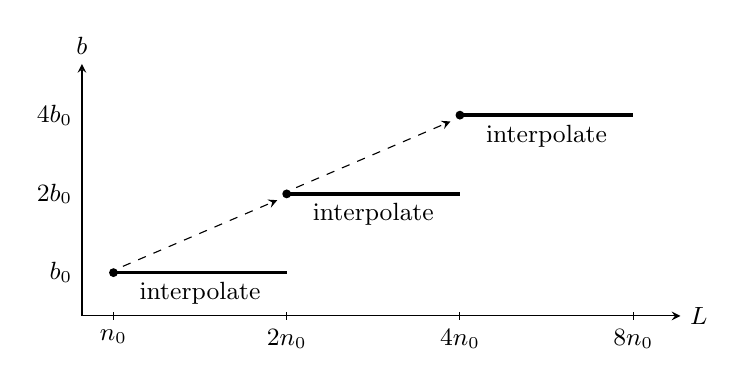
\begin{tikzpicture}[>=stealth, every node/.style={font=\small}]
 \draw[->] (-0.4,-0.55) -- (7.2,-0.55) node[right] {$L$};
 \draw[->] (-0.4,-0.55) -- (-0.4,2.65) node[above] {$b$};
 \foreach \x/\lab in {0/n_0,2.2/2n_0,4.4/4n_0,6.6/8n_0}
   {\draw (\x,-0.5)--(\x,-0.6);
    \node[below] at (\x,-0.6) {$\lab$};}
 \foreach \y/\lab in {0/b_0,1/2b_0,2/4b_0}
   {\node[left] at (-0.4,\y) {$\lab$};}
 \draw[very thick] (0,0)--(2.2,0);
 \draw[very thick] (2.2,1)--(4.4,1);
 \draw[very thick] (4.4,2)--(6.6,2);
 \fill (0,0) circle (1.6pt);
 \fill (2.2,1) circle (1.6pt);
 \fill (4.4,2) circle (1.6pt);
 \draw[->,dashed] (0.12,0.08)--(2.08,0.92);
 \draw[->,dashed] (2.32,1.08)--(4.28,1.92);
 \node[below] at (1.1,0) {interpolate};
 \node[below] at (3.3,1) {interpolate};
 \node[below] at (5.5,2) {interpolate};
\end{tikzpicture}
\caption{The bootstrap, shown schematically at three dyadic scales.
Dashed arrows double the starting length and inverse temperature.
At each scale, interpolation controls the physical purity for every
even length on the solid interval.  The intervals cover all larger
even lengths.}
\label{fig:bootstrap}
\end{figure}

\subsection{The two parameter choices}

We will establish the initial inequalities
\eqref{eq:bootstrap-seeds} for the following two rows:
\begin{equation}\label{eq:bootstrap-parameters}
\begin{array}{c|c|c|c|c}
 n_0&b_0&u_0&C&r=Cu_0\\ \hline
 60&105/4&1/8&79/10&79/80\\
 2304&784&1/100&5&1/20
\end{array}
\end{equation}
The scalar hypotheses of Proposition~\ref{prop:bootstrap} can already
be checked. For the first row,
\[
 G(1/8)=\frac{913952}{117649}<\frac{79}{10},\qquad
 \frac{3}{C(1-3u_0)}=\frac{48}{79}<1.
\]
For the second, $1-(1-u)^3\le3u$ gives, when $0<u\le1/100$,
\[
 G(u)\le\frac{9}{2(1-3u)^2}
 \le\frac{45000}{9409}<5,\qquad
 \frac{3}{C(1-3u_0)}=\frac{60}{97}<1.
\]
Thus the two rows give respectively the bounds
$(4/105)\log(80/79)$ and $(\log20)/784$ in
\eqref{eq:bootstrap-gap}, once their initial purities are proved.
The second row will follow from six applications of
Lemma~\ref{lem:rounded-update} to bounds based at $(36,49/4)$.
The remaining task is therefore finite: establish the two sets of
initial inequalities without losing the margins needed in these
updates.
